\chapter{Methodology}
\label{chp:methods}
This chapter presents the experimental methodology used throughout subsequent chapters. Firstly, the chapter describes a sensing system for collection of a large-scale unsupervised human gait data set. The chapter then presents the development of a data post-processing pipeline and a machine learning environment.

\section{Data Collection}
%------------------------------------------------------------------%
\subsection{Hardware}
A new set of first-hand gait data is required. To collect this required the development of a data collection system. The data set will comprise labelled gait data collected in an unsupervised manner from real-world environments. Therefore the system must be simple to operate unaided, portable, and non-intrusive. This section describes the development of a solution to fulfil these requirements.

A suitable recording platform is required to capture the gait data. The Suunto Movesense was selected because it is a low-cost (£70) \acrfull{cots} system that can be programmed to match user requirements. The Movesense contains a nine-axis \acrshort{marg} sensor, heart rate monitor, temperature sensor, and \acrshort{ble} radio. It is physically small, weighing just ten grams, and allows numerous attachment configurations.  Figure \ref{fig:methods-movesense-sensor} shows the Movesense device.

\begin{figure}[hbt]
    \centering
    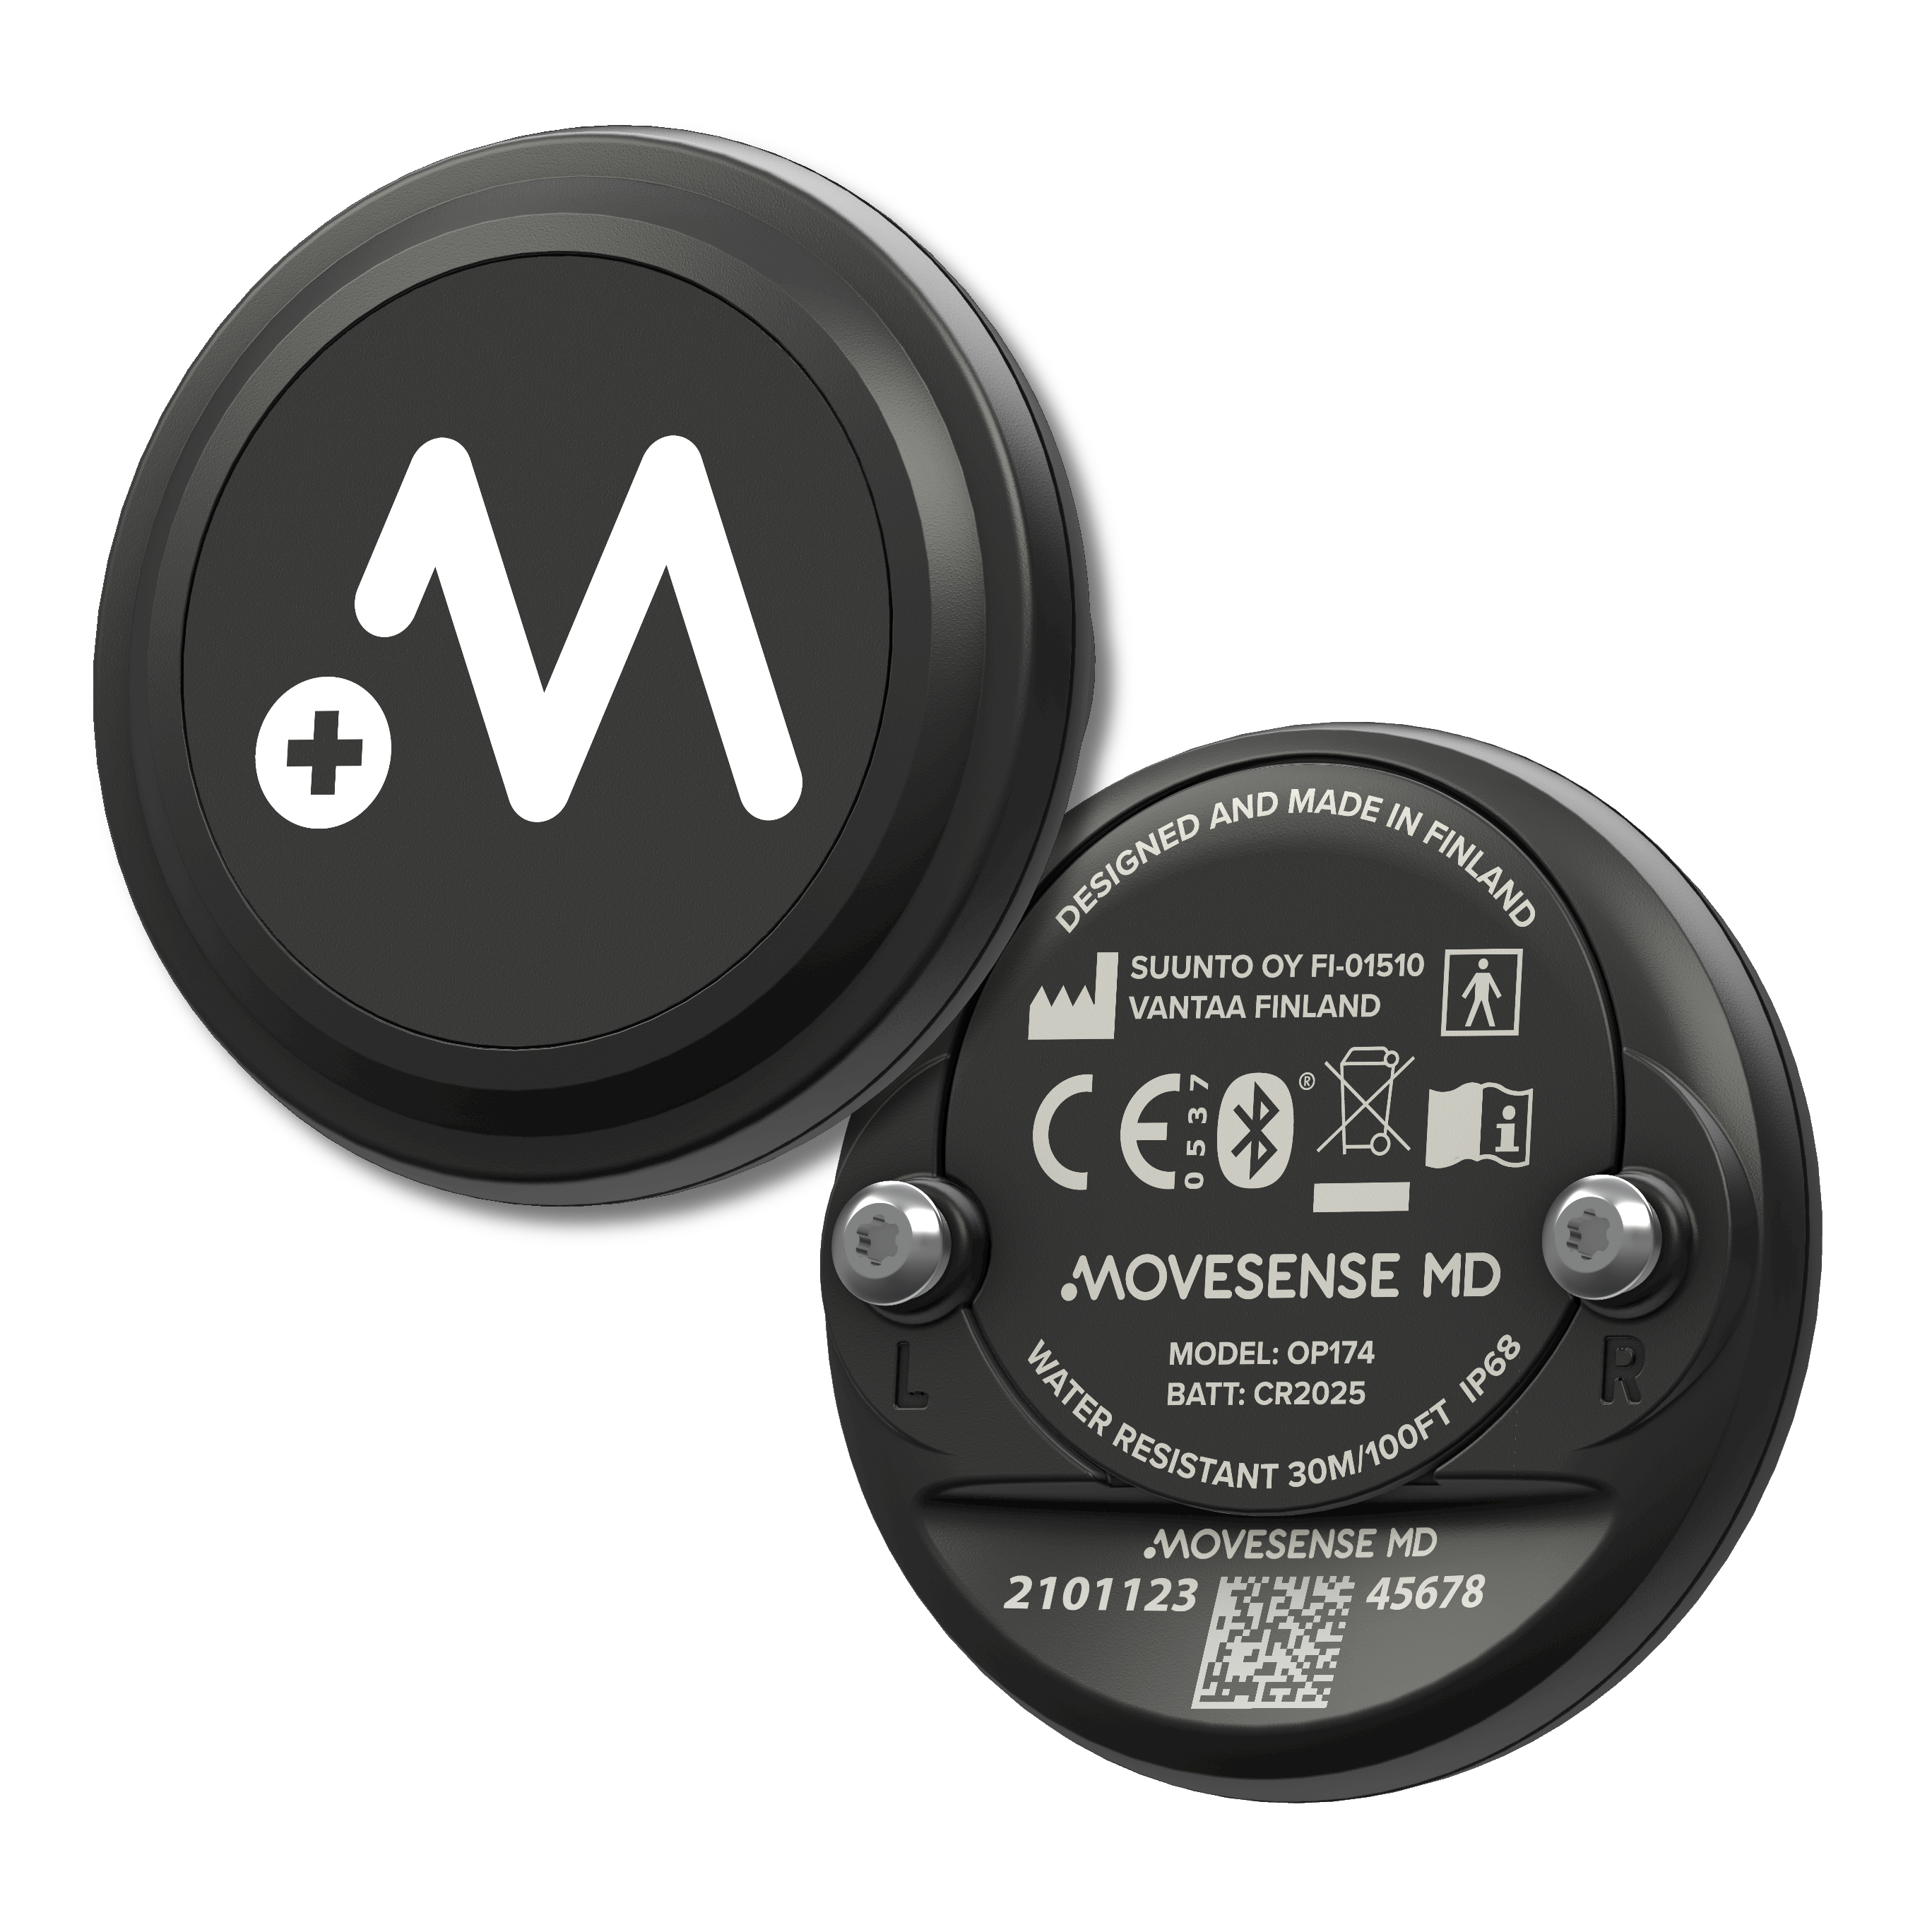
\includegraphics[width=0.5\textwidth]{content/3-Methods/Movesense-MD-front-and-back.png}
    \caption[Movesense Wearable IMU]{Movesense Wearable IMU\cite{movesensepress2022}}
    \label{fig:methods-movesense-sensor}
\end{figure}

The device's rear contact act as the mounting point for attaching the device using to wide variety of straps and clips, including a heart rate strap, belt clip and elasticated Velcro strap. Five sensors were attached to each participant in the following locations: on the inside of both ankles using an elastic Velcro strap, on~each hip using a clothes/belt clip and across the chest using a heart rate strap. The location of the sensors was selected to give broad coverage of body movements while providing easy, secure and non-invasive attachment to minimise discomfort and disruption to natural movement. Figure \ref{fig:methods-movesense-sensor-locations} shows a subject wearing the five sensors.

\begin{figure}[hbt]
    \centering
    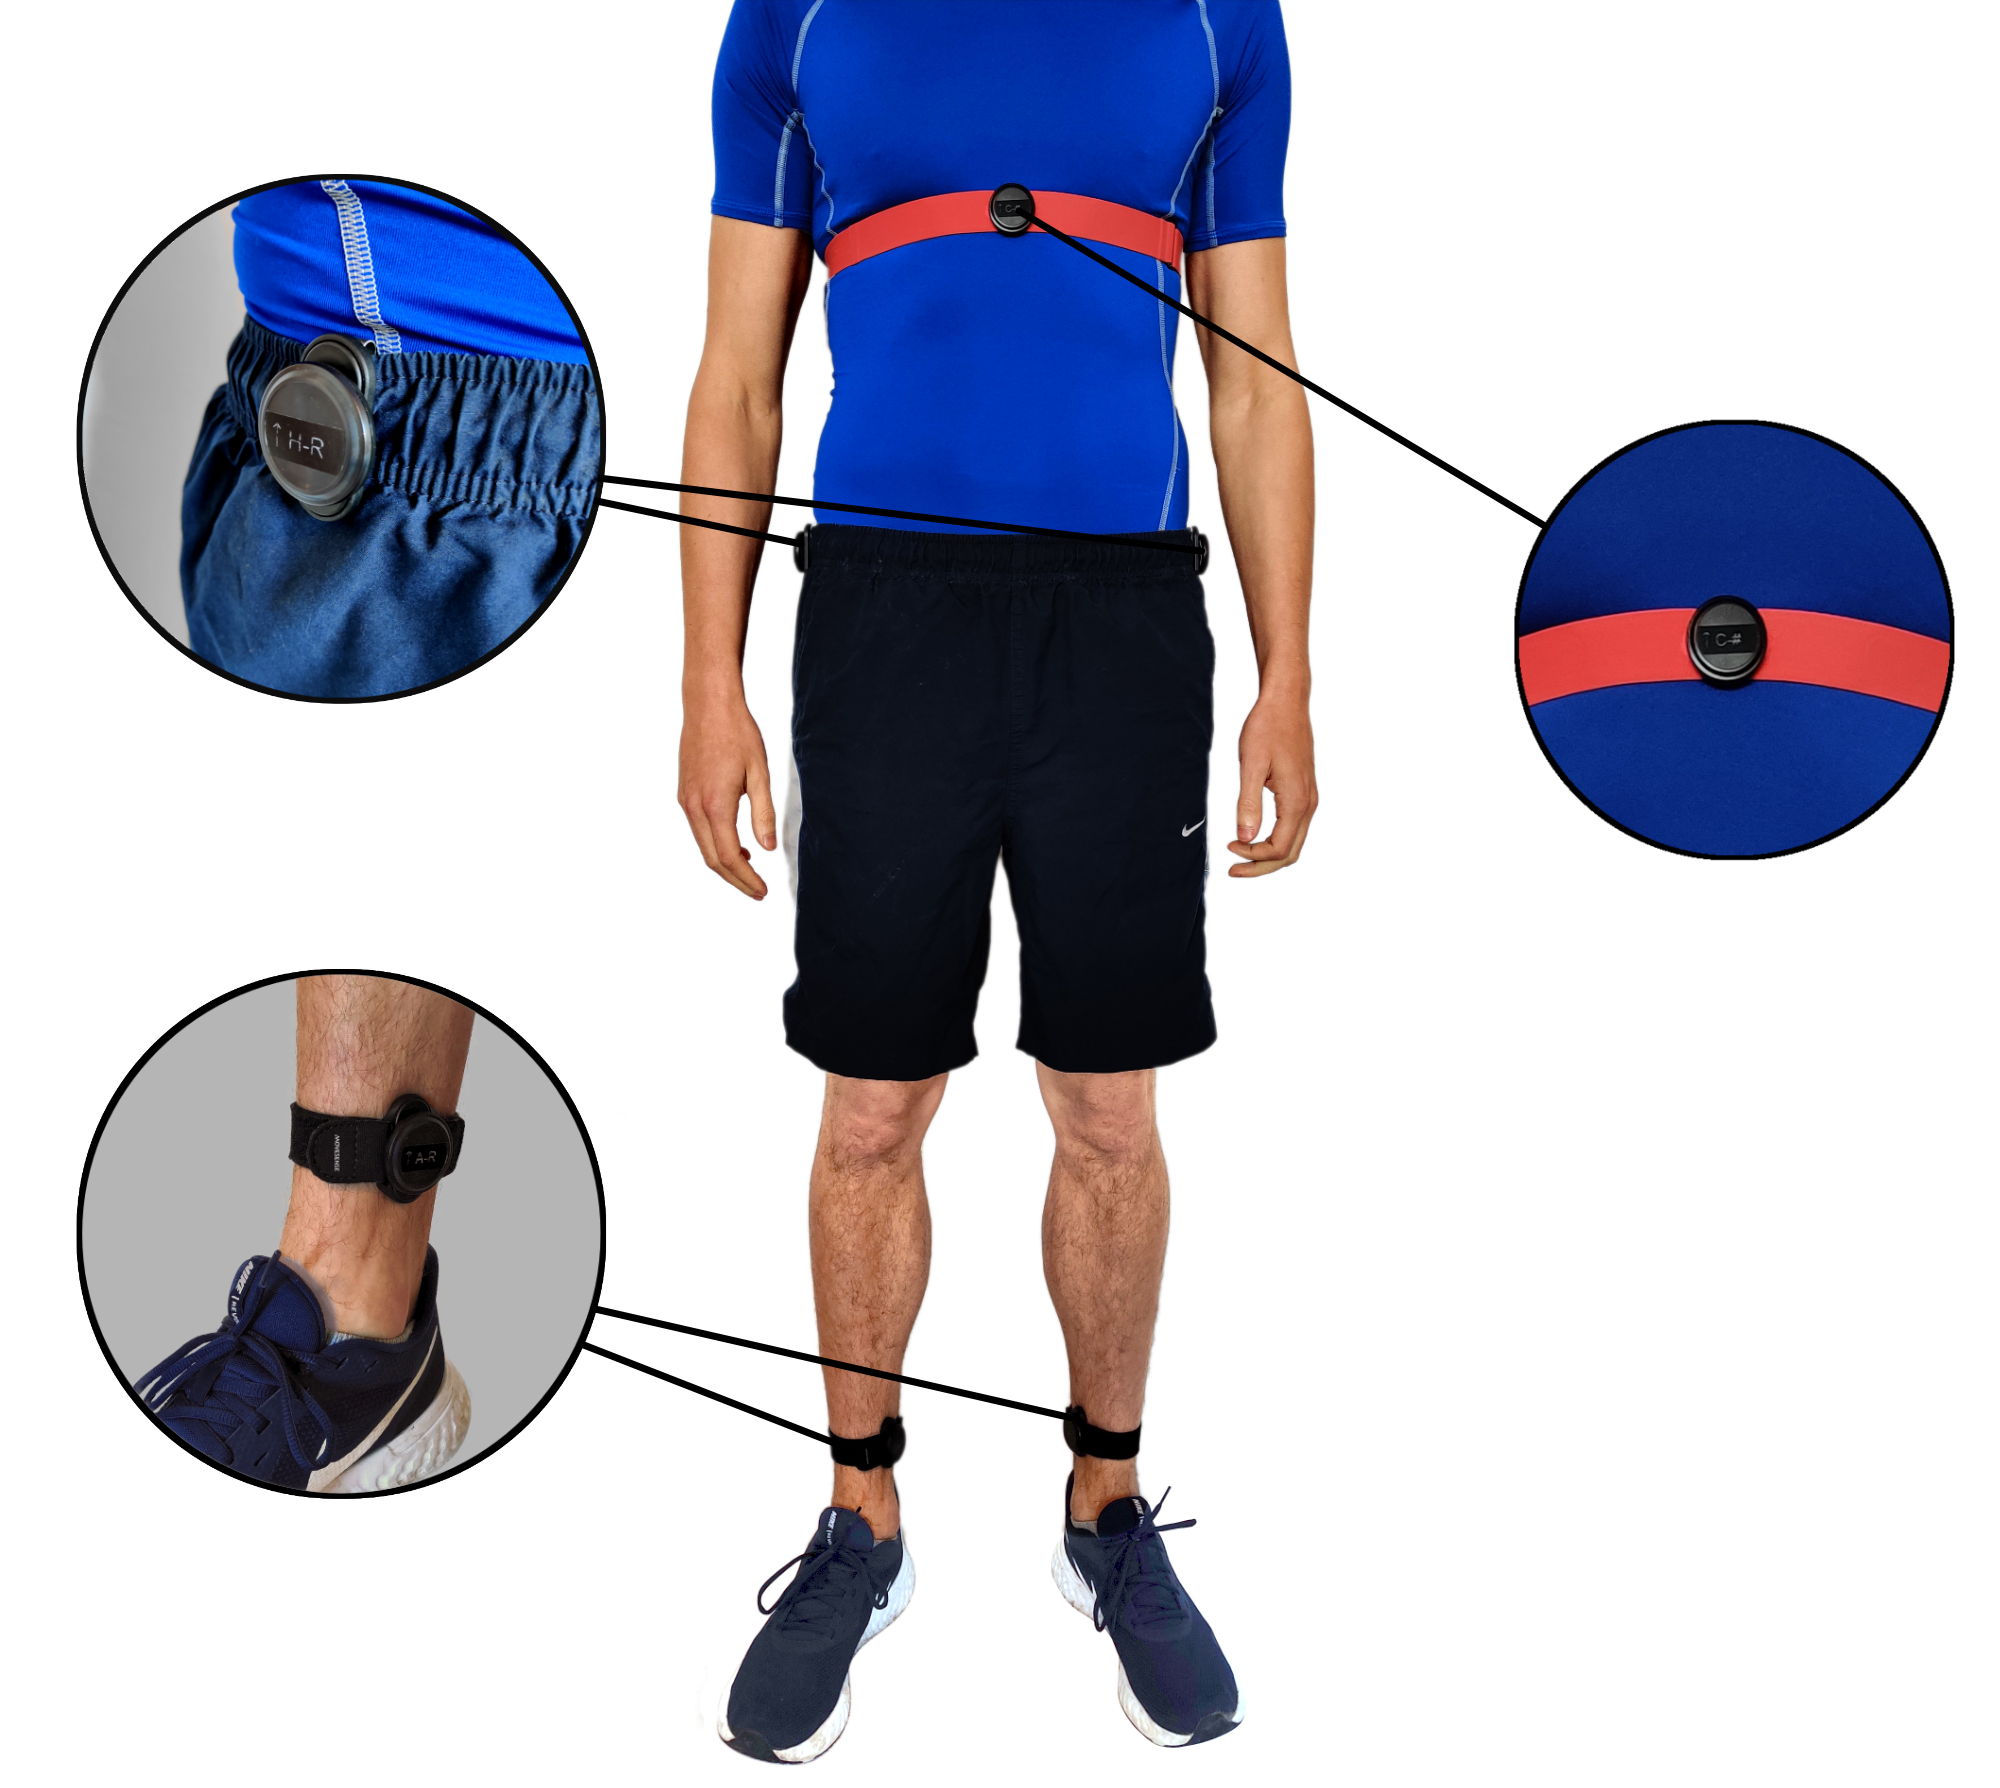
\includegraphics[width=0.6\textwidth]{content/3-Methods/sensor_locations.png}
    \caption{Movesense sensor attachment locations \cite{Sherratt2021}}
    \label{fig:methods-movesense-sensor-locations}
\end{figure}

The onboard MARG sensor is factory calibrated therefore no sensor calibration is required. Basic verification test were undertaken to ensure compliance with the manufacturer stated performance. A small coin cell battery powers the sensor, providing multiple hours of continuous operation. A configurable low power mode can extend the usable lifetime significantly.

Suunto provides an \acrfull{sdk} that allows developers to reprogram the Movesense customising its behaviour. A custom program transmitted live sensors readings over the inbuilt \acrshort{ble} radio. The transmitted data included the \acrshort{marg} heart rate and temperature sensors at 100Hz. An Android smartphone held by the test subject received this data through a custom data-logging application.

The software also implemented power management. By placing the sensors in an ultra-low power state when inactive, as detected by low readings of the accelerometer, the device can dramatically extend its battery life. The subject can wake the devices by touching both rear contacts. The power management system allowed for sharing of the sensors with trial subjects without worry about battery issues.


%--------------------------------------------------------
\subsubsection{BLE Data Transmission} % How is sensor data transmitted 
\label{subsection:methods-on-sensor-compression}
Data is transmitted from each Movesense wirelessly to a smartphone using the built-in \acrshort{ble} radio transceiver. Using the BLE notify mechanism, a custom \acrfull{gatt} service pushes data packets to a connected smartphone. Data streaming starts when the connected phone sets a notify state in the \acrshort{gatt} characteristic. Streaming stops once cleared. Clearing either occurs on \acrshort{ble} disconnection or programmatically. Data streaming is a high power state only entered during recording.

Two limits restrict the data rate that the sensor can transmit: maximum individual packet size and transmission rate. The maximum packet size is 155 bytes long. The practical limit of transmission rate is 15Hz, due to the need to transmit concurrently from five sensors. These limits require multiple IMU samples be transmitted per packet to achieve a real-time 100Hz output.

IMU data from the sensor arrives as a 32-bit floating-point number. Therefore each full sample of the nine-axis \acrshort{marg} sensor takes up 36 bytes. Uncompressed, the byte limit only allows for four samples; therefore, transmission requires data compression.

Compressing each measurement to a signed sixteen-bit fixed point integer allow for eight \acrshort{marg} measurements to be transmitted per packet. To achieve compression, each raw value is multiplied by a scaling factor before typecast to a sixteen-bit integer. This compression technique retains the sub-decimal accuracy while allowing for sufficient compression. Table \ref{tab:methods-imu-data-compression-factors} presents the sensor ranges, scaling factors and resultant accuracy of each sensor. As sixteen-bit integer values have a maximum range of -32,768 to 32,767, clipping will occur if the typecast value of the sensors exceeds these limits. The chosen scaling factor was a balance between accuracy and output range. The calculation of output range requirement was empirical.

\begin{table}[hbt]
    \centering
    \caption[Compression of sensor readings, scaling factors and resultant accuracies]{Compression of sensor readings, scaling factors and resultant accuracies. Force of Gravity (g), \acrfull{dps}, MicroTesla ($\mu T$)} % Fix caption units should be defined else where
    \label{tab:methods-imu-data-compression-factors}
    
    \begin{tabularx}{\textwidth}{Y|YYY}
        \noalign{\hrule height 1.5pt}
        \textbf{Sensor} & \textbf{Sensor Range} & \textbf{Scaling Factor} & \textbf{Accuracy} \\
        \hline
        Accelerometer & $\pm16 g$ & $256$ & $\pm0.039 g$ \\
        Gyroscope & $\pm2000 DPS$ & $32$ & $\pm0.031 DPS$ \\
        Magnetometer & $\pm5000\mu T$ & $1$ & $\pm1\mu T$ \\
        \noalign{\hrule height 1.5pt}
    \end{tabularx}
\end{table}

When compressed, eight \acrshort{marg} samples fit within one packet leaving eleven bytes available. These final bytes contain a timestamp based on the internal sensor clock, sensor temperature, heart rate, and R-R interval. The addition of these was in case of future use. Temperature, heart rate and R-R interval are only updated when they change value. The remaining byte contains an update flag for each field. Figure \ref{fig:methods-ble-packet-structure} shows the entire 155-byte transmission packet.

\begin{figure}[hbt]
    \centering
    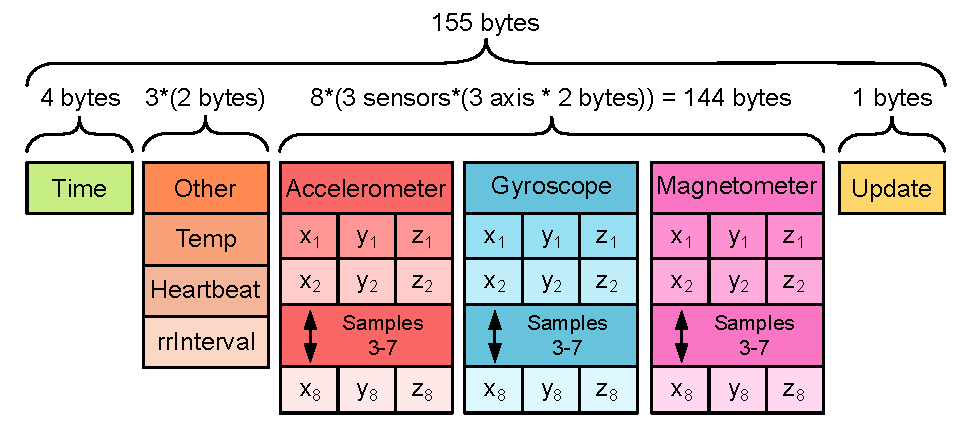
\includegraphics[width=0.9\textwidth]{content/3-Methods/BLE_Bytes_Packets.pdf}
    \caption[Movesense \glsentrylong{ble} transmission packet structure]{Movesense \acrlong{ble} transmission packet structure}    \label{fig:methods-ble-packet-structure}
\end{figure}


%--------------------------------------------------------
\subsubsection{Android Application}
The android application serves three purposes: to save the sensor data, annotate the current activity, and share annotated data with researchers. The app runs on a smartphone carried by the test subject.

The application's user interface is intentionally simple, requiring minimal instruction to use. Figure \ref{fig:methods-app-user-interface} shows the application user interface in all states.

\begin{figure}[hbt]
    \centering
    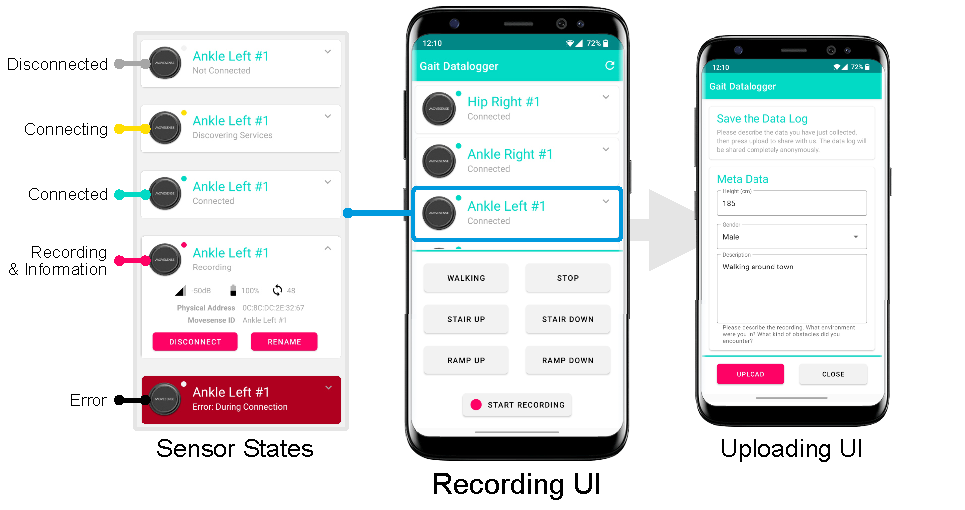
\includegraphics[width=\textwidth]{content/3-Methods/User_Interface.pdf}
    \caption{Data-logging android application user interface.}
    \label{fig:methods-app-user-interface}
\end{figure}

When the application opens, it automatically connects to the detected sensors. This process can also be run manually by pressing the refresh button or dragging and releasing the list of devices. All detected devices show their current connection and activity states through a connection state icon and large status text. Any sensor errors are clearly shown by highlighting the sensor in red and displaying error text.

Recording begins when the test subject presses the large `start recording' button at the bottom of the screen. All connected sensors begin transmitting data—their reported status changes to recording along with a red dot icon. The onboard LED of each sensor also flashes red providing a physical indication.

When the subject presses the record button, the notify state is set on each device, starting data streaming. The BLE service passes received data to the file saving service. This service creates plain text files locally on the phone. Sensor messages are each saved on a new line containing the sensor byte data, encoded as a hexadecimal string, the smartphone's timestamp, and the sensors MAC address.

When the test subject presses the `stop recording` button recording stops. The app then presents the user with an upload screen. The upload screen allows metadata entry and anonymously sharing data through Google Firebase cloud services.

Figure \ref{fig:methods-android-app} illustrates the interactions between each different aspect of the android application.

\begin{figure}[hbt]
    \centering
    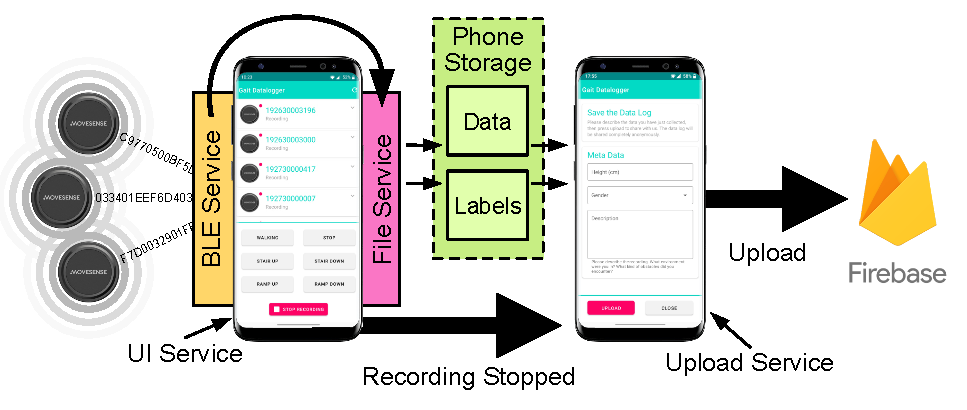
\includegraphics[width=0.9\textwidth]{content/3-Methods/Android_App.pdf}
    \caption{Data-logging Android App}
    \label{fig:methods-android-app}
\end{figure}


%------------------------------------------------------------%
\subsection{Collection Methods}
\label{sec:methods-data-collection}
An extensive set of gait data is required to develop \acrshort{ml} systems for classifying locomotive mode. The gait data should be from a real-world unstructured environment which includes common imperfections and disturbances. The data will be collected using the Movesense sensors described previously. The study received ethical approval from the University of Bath Research Ethics Approval Committee for Health (REACH), reference \textit{EP 19/20 003}.

%----------------------------------------------------------------
\subsubsection{Activities}
The following activities were selected, Walking, \acrfull{sa}, \acrfull{sd}, \acrfull{ra}, \acrfull{rd}) and Stopped. Labarri\`ere et al. identified these as the most commonly investigated as they require no equipment or skill to perform\cite{Labarriere2020}. The collection of these activities will be in the real world. Figure \ref{fig:methods-example-enviroments} shows examples of the environments for data was collected.

% Pictures showing the variety of terrain %
\begin{figure}[!hbtp]
     \centering
     \begin{subfigure}[b]{\textwidth}
         \centering
         \begin{subfigure}[b]{0.32\textwidth}
             \centering
             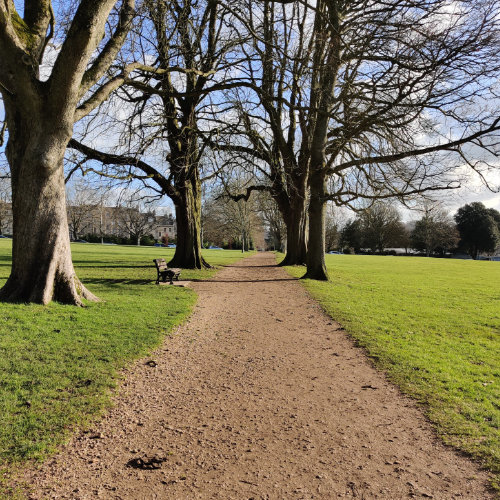
\includegraphics[width=\textwidth]{content/3-Methods/enviroments/flat_1_modified.jpg}
        \end{subfigure}
        \hfill
         \begin{subfigure}[b]{0.32\textwidth}
             \centering
             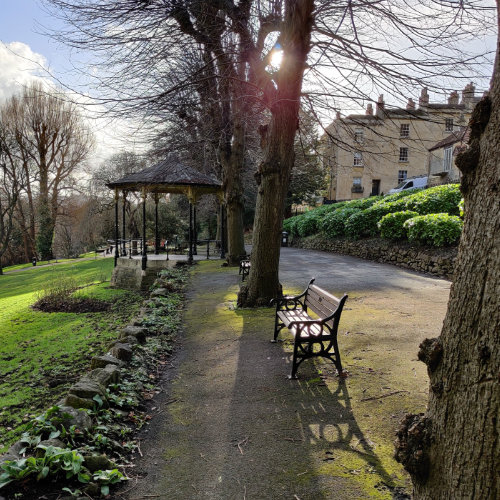
\includegraphics[width=\textwidth]{content/3-Methods/enviroments/flat_2_modified.jpg}
        \end{subfigure}
        \hfill
        \begin{subfigure}[b]{0.32\textwidth}
             \centering
             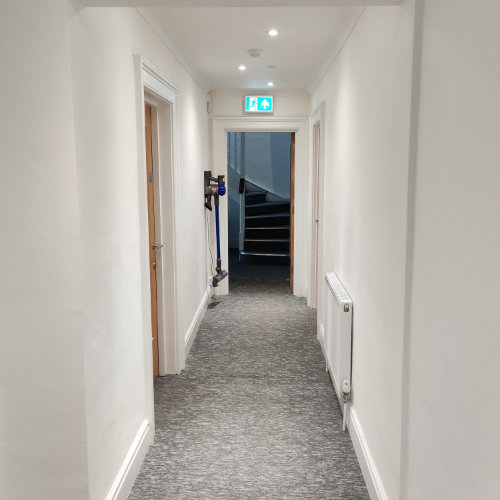
\includegraphics[width=\textwidth]{content/3-Methods/enviroments/flat_3_modified.jpg}
        \end{subfigure}
        \caption{Walking}
        \label{fig:methods-flat-example}
      \end{subfigure}
      \newline
      
      \begin{subfigure}[b]{\textwidth}
         \centering
         \begin{subfigure}[b]{0.32\textwidth}
             \centering
             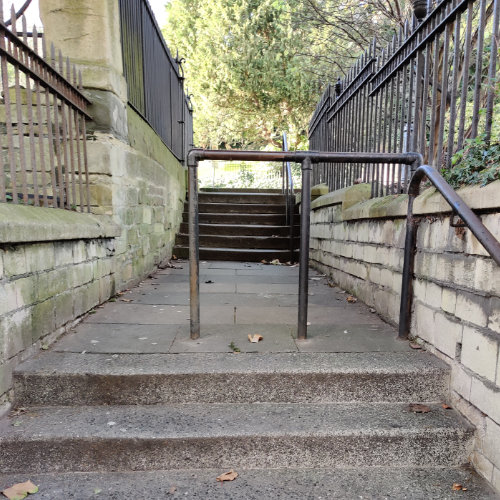
\includegraphics[width=\textwidth]{content/3-Methods/enviroments/stair_1_modified.jpg}
        \end{subfigure}
        \hfill
         \begin{subfigure}[b]{0.32\textwidth}
             \centering
             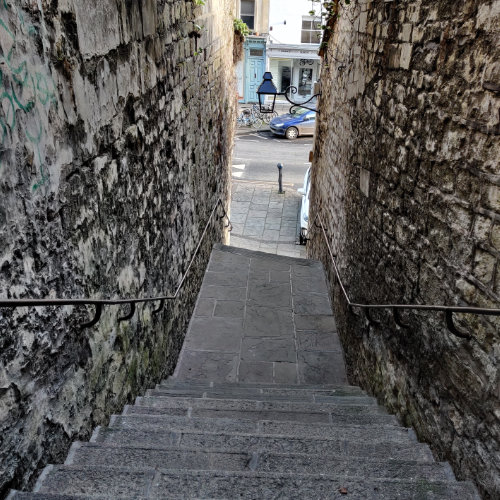
\includegraphics[width=\textwidth]{content/3-Methods/enviroments/stair_2_modified.jpg}
        \end{subfigure}
        \hfill
        \begin{subfigure}[b]{0.32\textwidth}
             \centering
             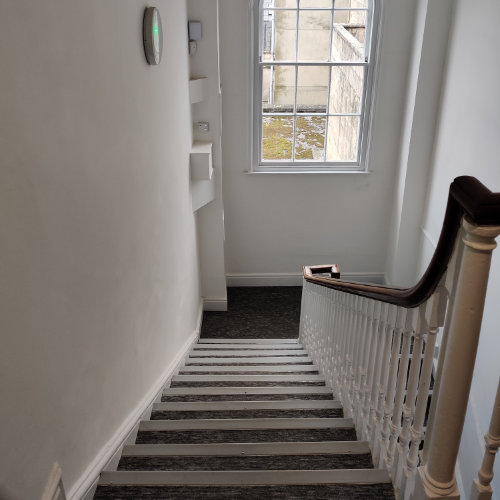
\includegraphics[width=\textwidth]{content/3-Methods/enviroments/stair_3_modified.jpg}
        \end{subfigure}
        \caption{Stairs}
        \label{fig:methods-stair-example}
      \end{subfigure}
      \newline
      
      \begin{subfigure}[b]{\textwidth}
         \centering
         \begin{subfigure}[b]{0.32\textwidth}
             \centering
             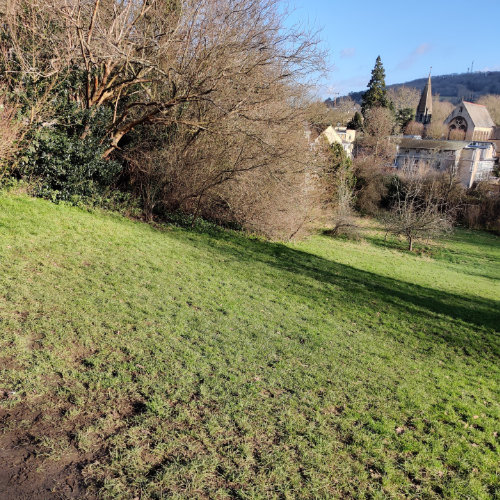
\includegraphics[width=\textwidth]{content/3-Methods/enviroments/ramp_1_modified.jpg}
        \end{subfigure}
        \hfill
         \begin{subfigure}[b]{0.32\textwidth}
             \centering
             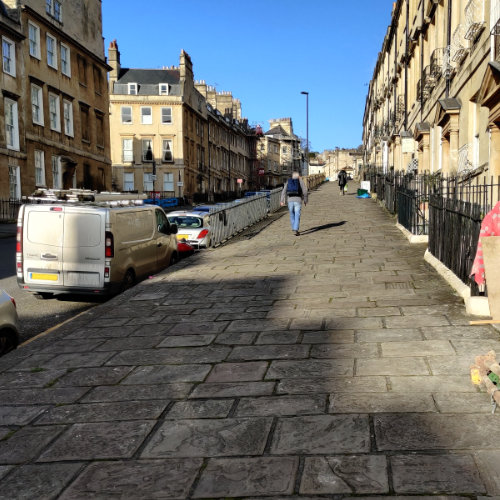
\includegraphics[width=\textwidth]{content/3-Methods/enviroments/ramp_2_modified.jpg}
        \end{subfigure}
        \hfill
        \begin{subfigure}[b]{0.32\textwidth}
             \centering
             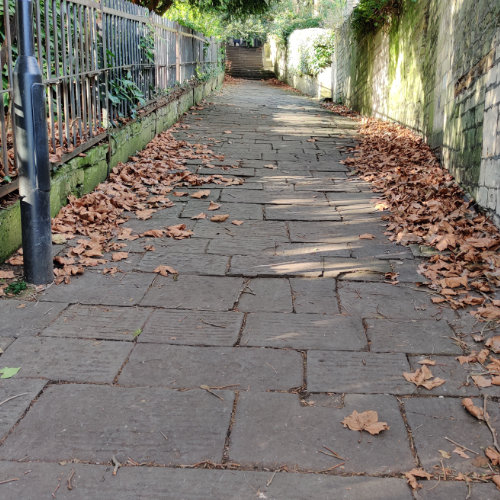
\includegraphics[width=\textwidth]{content/3-Methods/enviroments/ramp_3_modified.jpg}
        \end{subfigure}
        \caption{Ramp/Hill}
        \label{fig:methods-ramp-example}
      \end{subfigure}
    \caption{Example of data recording environments}
    \label{fig:methods-example-enviroments}
\end{figure}

%----------------------------------------------------------------
\subsubsection{Recording Procedure} % How were the subjects instructed to label data - press at first HS on new activity
Study subjects received instructions on using sensing equipment and general guidance on experiment procedures. The guidance comprised general guidance to walk around a varied environment while labelling the six activity classes. Study subjects received no further instructions on recording conduct.

% %----------------------------------------------------------------
% \subsection{Summary of Data Collected} %TODO Expand on this section
% A brief summary of the data collected over the course of this research is presented below.

% Data was collected in three phases:
% \begin{enumerate}
%     \item Large number of non-amputee participants - limited data per participant
%     \item Small number of non-amputee participants - extensive data per participant
%     \item Data from amputees
% \end{enumerate}

% The first phase of data collection focused of collecting from a broad range of individuals in different environments. Table \ref{tab:methods-phase-1-data-summary} contains a summary of the data collected during the first phase of data collection. Data was collected from twenty-two participants of a wide variety of age (mean 29, std 10), gender (17 male, 5 female), and physique.

% The second phase of data collection involved the collection of data from a smaller number of individuals but with a focus on collecting at least seven minutes of data for each activity. Table \ref{tab:methods-phase-2-data-summary} show a summary of the data collected during the second phase. Data was collected from three subjects, two males aged 25 and 27, and one female of age 26.

% % Third round of data collection
% The third stage of data collection focused on collecting data from amputees. Table \ref{tab:methods-phase-3-data-summary} contains a summary of the first hand data collected during this phase. The data was for one left trans-tibial individual.

% \begin{table}[p]
%     \centering
%     \caption[Data samples of non-amputee data collected during the first phase of collection]{Summary of non-amputee data collected during the first phase of collection. (\acrfull{ra}, \acrfull{rd}, \acrfull{sa}, \acrfull{sd})}
%     \label{tab:methods-phase-1-data-summary}
%     %W---Walking, RA---Ramp Ascent, RD---Ramp Descent, SA---Stair Ascent, SD---Stair Descent, S---Stopped
%     \begin{tabularx}{\textwidth}{c|YYYYYY}
%       \noalign{\hrule height 1.5pt}
%       \textbf{Subject ID} & \textbf{WALK} & \textbf{\glsentryshort{ra}} & \textbf{\glsentryshort{rd}} & \textbf{\glsentryshort{sa}} & \textbf{\glsentryshort{sd}} & \textbf{STOP} \\
%       \hline
%         01 & 34618 & 0 & 0 & 5349 & 5025 & 1281 \\
%         02 & 13564 & 0 & 0 & 4614 & 4447 & 1020 \\
%         03 & 5005 & 0 & 0 & 3633 & 2568 & 1587 \\
%         04 & 32336 & 0 & 0 & 6045 & 5482 & 0 \\
%         05 & 32525 & 0 & 0 & 6621 & 5767 & 0 \\
%         06 & 37895 & 0 & 0 & 8424 & 5636 & 0 \\
%         07 & 21843 & 0 & 0 & 14074 & 10873 & 0 \\
%         08 & 38590 & 0 & 0 & 11036 & 17801 & 0 \\
%         09 & 40384 & 0 & 0 & 10826 & 7953 & 0 \\
%         10 & 37353 & 0 & 0 & 10812 & 8084 & 0 \\
%         11 & 8341 & 0 & 0 & 1614 & 1566 & 0 \\
%         12 & 9038 & 0 & 0 & 6273 & 4926 & 0 \\
%         13 & 252022 & 48821 & 53735 & 18778 & 16220 & 16887 \\
%         14 & 302440 & 18531 & 18305 & 10936 & 9581 & 73781 \\
%         15 & 12249 & 0 & 0 & 1452 & 1929 & 3498 \\
%         16 & 23729 & 0 & 0 & 5332 & 2578 & 1651 \\
%         17 & 113222 & 2702 & 3754 & 3190 & 3949 & 19127 \\
%         18 & 37352 & 0 & 0 & 3747 & 2565 & 1133 \\
%         19 & 4990 & 0 & 0 & 1240 & 1245 & 0 \\
%         20 & 3487 & 0 & 0 & 2383 & 3054 & 0 \\
%         21 & 4806 & 0 & 0 & 2551 & 190 & 206 \\
%         22 & 9033 & 3274 & 3630 & 982 & 938 & 856 \\
%         \hline
%         \textbf{Total} & 1075111 & 73328 & 79426 & 139915 & 122378 & 121027 \\
%         \noalign{\hrule height 1.5pt}
%     \end{tabularx}
% \end{table}

% \begin{table}[p]
%     \centering
%     \caption[Data samples of non-amputee data collected during the second phase of collection]{Data samples of non-amputee data collected during the second phase of collection. (\acrfull{ra}, \acrfull{rd}, \acrfull{sa}, \acrfull{sd})}
%     \begin{tabularx}{\textwidth}{c|YYYYYY}
%       \noalign{\hrule height 1.5pt}
%       \textbf{Subject ID} & \textbf{WALK} & \textbf{\glsentryshort{ra}} & \textbf{\glsentryshort{rd}} & \textbf{\glsentryshort{sa}} & \textbf{\glsentryshort{sd}} & \textbf{STOP} \\
%       \hline
%       01 & 462446 & 141268 & 139786 &59685 & 44024 & 62397 \\
%       03 & 291213 & 77508 & 59157 & 48695 & 50210 & 157867 \\
%       09 & 368090 & 115299 & 82980 & 49530 & 51698 & 60605 \\
%       \hline
%       \textbf{Total} & 2100308 & 404127 & 364574 & 277250 & 252494 & 363669 \\
%       \noalign{\hrule height 1.5pt}
%     \end{tabularx}
%     \label{tab:methods-phase-2-data-summary}
% \end{table}
% % Amputee data
% \begin{table}[p]
%     \centering
%     \caption[Data samples of first hand amputee data collected during the third phase of collection]{Data samples of first hand amputee data collected during the third phase of collection. (\acrfull{ra}, \acrfull{rd}, \acrfull{sa}, \acrfull{sd})}
%     \begin{tabularx}{\textwidth}{c|YYYYYY}
%       \noalign{\hrule height 1.5pt}
%       \textbf{Subject ID} & \textbf{WALK} & \textbf{\glsentryshort{ra}} & \textbf{\glsentryshort{rd}} & \textbf{\glsentryshort{sa}} & \textbf{\glsentryshort{sd}} & \textbf{STOP} \\
%       \hline
%       A1 & 38114 & 6159 & 7194 & 2872 & 2450 & 11763 \\
%       \noalign{\hrule height 1.5pt}
%     \end{tabularx}
%     \label{tab:methods-phase-3-data-summary}
% \end{table}

% % Discussion about collected data
% What is unique about our data set
% \begin{itemize}
%     \item Unsupervised (no researcher bias in activity pattern) - subject Provided with sensors, app and basic instructions of how to setup and label data
%     \item Wide range of different natural environments and terrain
%     \item Large number of people
%     \item Comparable data from an amputee
% \end{itemize}

% Systematic issues with the data set
% \begin{itemize}
%     \item Poorly distributed classes - real life distribution of activities is not even. Walking and hills/ramps are far more prevalent than stairs.
%     \item Label noise due to likely inconsistencies between individuals when collecting data
%     \item Different amounts of data for different participants
% \end{itemize}


%------------------------------------------------------------------%
\section{Data Post-Processing}
Data processing is necessary to prepare the raw recorded data for use in a machine learning environment. Within this section, the methods used to accomplish this transformation are detailed.

% Terminology
The data collected can be described by the hierarchical structure in Figure \ref{fig:methods-data-hierachy}. Each participant has a series of gait data recordings. Each recording contains live annotation made using the android app. Recordings likely contain different distributions of activities, each from a different environment. Each continuous period of an activity label is an episode of data. So a recording is made up of a series of contiguous episodes of data. The period around a change in the episode is a transition between activities. In the dataset, the labels represent this as a discrete change, but, in reality, it would be a smooth easing between locomotive modes.

\begin{figure}[hbt]
    \centering
    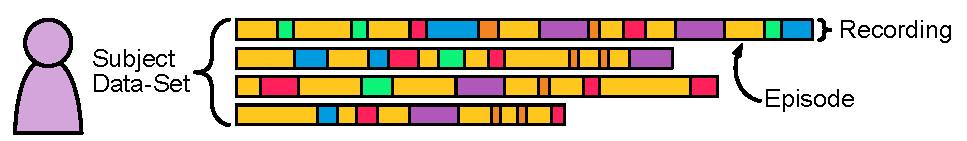
\includegraphics[width=0.9\textwidth]{content/3-Methods/Data_Terminology.pdf}
    \caption{The hierarchical structure of the data recordings and terminology.}
    \label{fig:methods-data-hierachy}
\end{figure}

%Issues with the data
Two \acrfull{etl} scripts prepare the data for \acrshort{ml} and address systematic issues with the data. An \acrshort{etl} is a common technique in data science for copying data from one or more sources to a new destination where a different representation is required. An \acrshort{etl} script written in Matlab 2019b transforms the sensor data from its raw form to \acrshort{csv} files for import into a Python environment. The second \acrshort{etl} script, written in Python, prepares the data for loading into the machine learning environment. The remainder of this section presents a more detailed description of both two scripts.

\subsection{Sensor Data ETL}
\label{subsec:sensor-ETL}
The sensor data \acrshort{etl} script transforms raw sensor data into \acrshort{csv} tables for import into Python. Figure \ref{fig:methods_sensor_ETL} illustrates the complete \acrshort{etl}.

\begin{figure}[hbt]
    \centering
    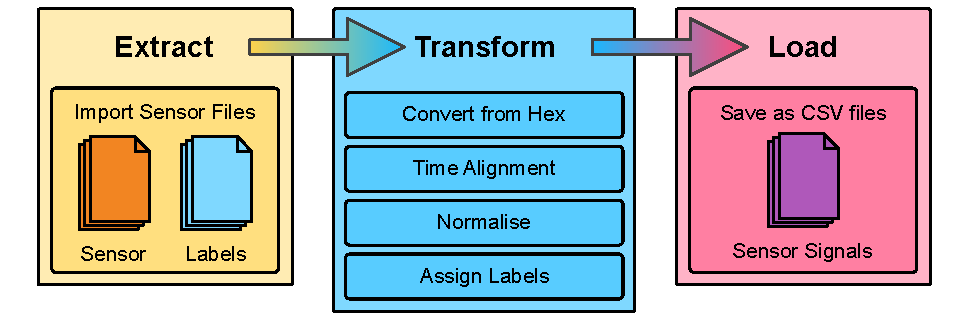
\includegraphics[width=0.9\textwidth]{content/3-Methods/Sensor_ETL.pdf}
    \caption{Flow Diagram of Sensor Data \acrshort{etl} process}
    \label{fig:methods_sensor_ETL}
\end{figure}

\subsubsection{Extract} % Extract - retrieving data from source
Each recording produces three files; a data file, label file and meta-data file. The three files contain the following:
\begin{itemize}
    \item \textbf{Data File} -- Encoded sensor data along with the smartphone timestamp
    \item \textbf{Label File} -- Activity labels and timestamps.
    \item \textbf{Meta File} -- Notes about the recording, such as participant height, gender and a brief unstructured recording description. The metadata does not form part of the ETL output.
\end{itemize}

Each sub-directory is opened and processed one at a time in order of recording date.

\subsubsection{Transform}
% Transform
The saved sensor data is in a hexadecimal encoding, with each pair of characters representing one byte of the sensor transmission data. The first operation is converting each pair of characters into its binary form. Then sets of binary values are typecast to integer values before applying the appropriate scalars to convert back to their original 32-bit floating-point representation. The conversion is the reverse of the on-sensor compression described previously.

Each line of sensor data contains the sensor's physical/MAC address. Files can be split into individual sensors using the MAC address. Before combining the individual sensors into a single data table, inconsistencies between the devices need to be corrected.

The sensors do not have onboard real-time clocks, with the sensor timestamp based upon the internal sensor clock. There is sufficient variation between each sensor that clock drift must be corrected. Calculations for long term drift come from comparing the sensor and smartphone timestamps. This drift is assumed to be linear; therefore, the correction offset and gain can be calculated using linear regression. Figure \ref{fig:methods-clock-drift-correction} shows an example of drift correction.

\begin{figure}[hbt]
    \centering
    \begin{subfigure}{0.45\textwidth}
         \centering
         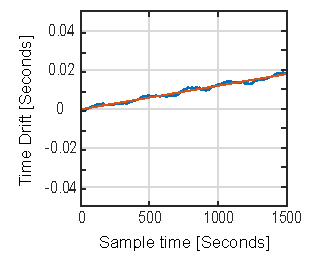
\includegraphics[width=0.95\textwidth]{content/3-Methods/Clock_Drift.pdf}
         \caption{Before correction}
    \end{subfigure}
    \begin{subfigure}{0.45\textwidth}
         \centering
         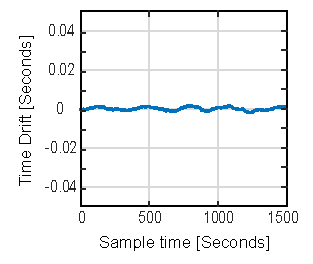
\includegraphics[width=0.95\textwidth]{content/3-Methods/Clock_Drift_Corrected.pdf}
         \caption{After correction}
    \end{subfigure}
    \caption{Example of sensor clock drift correction.}
    \label{fig:methods-clock-drift-correction}
\end{figure}

Each data packet contains eight sensors readings but only one timestamp. Therefore timestamps for each reading needs to be augmented. The augmented timestamps assumed a constant recording frequency.

Finally, the data is resampled to exactly 100Hz to ensure data for each sensor aligns correctly. Resampling was necessary because inconsistency in sensor clocks resulted in actual device sample rates varying by a couple of Hertz. The built-in Matlab resampling function was used for this. The Matlab function uses a spline function to calculate the interpolated value. At this point, the data from individual sensors can be combined into a single data table.

Data normalisation is an essential pre-processing step involving scaling features to a consistent range so that greater numeric feature values cannot dominate the smaller features\cite{Singh2020}. The main aim is to minimise the bias of those features whose numerical contribution is higher in discriminating pattern classes.

The last step involves applying activity labels to the data lines. The data labels recorded in the label file are aligned based on the smartphone's clock. The label for each table row is set by the last activity label encountered.

\subsubsection{Load}
Two saving options were employed:
\begin{itemize}
    \item Saving the complete recording as a single file
    \item Splitting the recording up into different files for each episode of an activity
\end{itemize}

Data tables are exported into \acrshort{csv} files, with files for each participant stored in separate folders. Basic statistics about each file include the number of samples of each activity and step count are also generated.

%--------------------------------------------%
\subsection{Machine Learning ETL}
\label{subsec:ML-ETL}
The second \acrshort{etl} script ingests the \acrshort{csv} data files previously generated and converts and prepares them for loading into a Tensorflow \acrshort{ml} environment. Tensorflow requires three sets of data, train, test, and validation, each presented as a set of data inputs along with a corresponding expected output. The \acrshort{etl} script was implemented in Python 3.8. Figure \ref{fig:methods_ml_ETL} shows a diagram of the \acrshort{etl} process.

\begin{figure}[hbt]
    \centering
    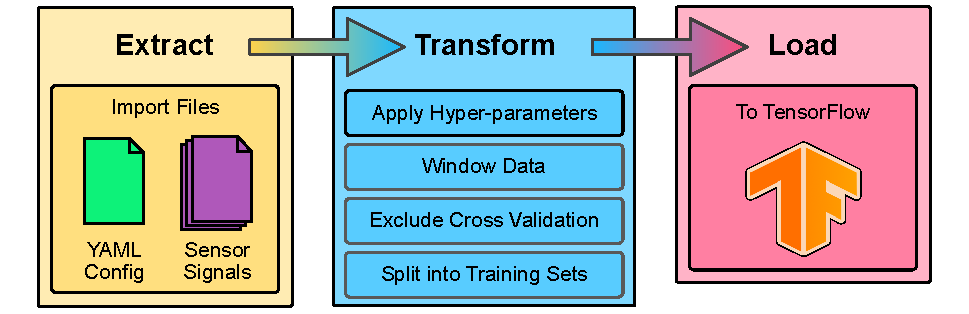
\includegraphics[width=0.9\textwidth]{content/3-Methods/ML_ETL.pdf}
    \caption[Flow Diagram of the \glsentrylong{ml} \glsentryshort{etl} process]{Flow Diagram of the \acrlong{ml} \acrshort{etl} process.}
    \label{fig:methods_ml_ETL}
\end{figure}

% Export
\subsubsection{Extract}
The \acrshort{etl} script accepts a \acrshort{yaml} configuration file. This file contains the configuration for the machine learning experiment. \acrshort{yaml} files allow experiments to be replicated easily by storing the experiment set up with the input data and results. The \acrshort{etl} script also supports a \acrshort{yaml} file to specify a range of values for any parameter for hyper-parameter sweeping.

The extract imports the \acrshort{etl} files previously generated from a directory specified in the configuration file using the Python library Pandas. The imported data is represented in Pandas data tables stored in memory, mapped to their associated participant and activity.
 
\subsubsection{Transform}
Hyper-parameters extracted from the \acrshort{yaml} file are used across all aspects of the transformation process to define constants.

The \acrshort{yaml} setup file specifies the columns of data that are required, for example, \textit{right-ankle-gyro-y}. These data columns are extracted from the Pandas data tables, with the remaining data discarded.

Each data window contains rows of data equal to the window size. Data for each window is copied from the table to form a new table. The window selection starts at the beginning of the data table. The window starting point is moved forward by a specified skip value for each new window resulting in a set of overlapping windows. Figure 1  \ref{fig:methods-data-window-generation} illustrates the data windowing process.

\begin{figure}[hbt]
    \centering
    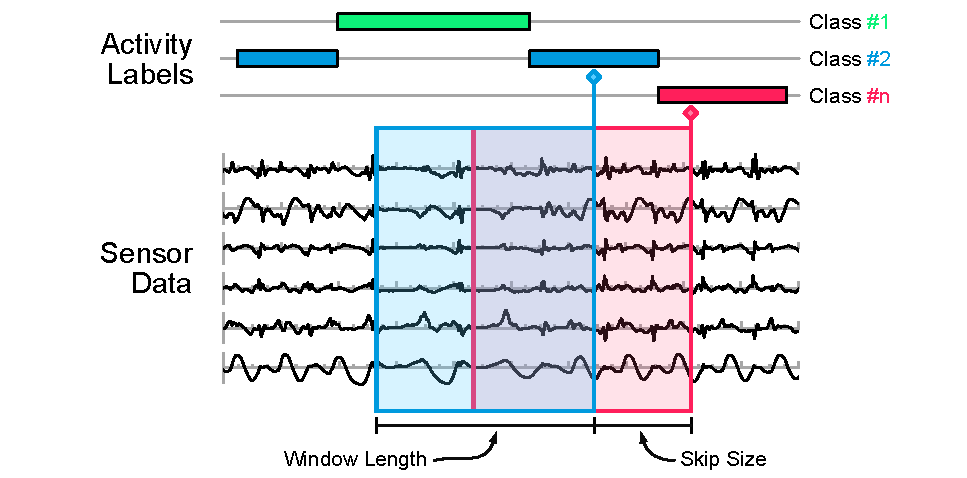
\includegraphics[width=0.9\textwidth]{content/3-Methods/Sliding_Window.pdf}
    \caption{Sliding window generation}
    \label{fig:methods-data-window-generation}
\end{figure}

The activity labels must be provided in the same output scheme as the \acrshort{ml} model; the output format is one-hot encoding. One-hot encoding gives each activity label an element in an array. The label array element is given a value of one; all other elements have a value of zero.

The windowed and labelled data must be split into three datasets, test, training and validation. How this is achieved will be experiment dependent; therefore, it will be discussed in the methods before each experiment.

\subsubsection{Load}
Finally, the three sets of windowed and labelled data are fed into TensorFlow. How TensorFlow is configured to process the transformed data is explained next.


\section{Machine Learning Methods}
%\cite{https://www.tensorflow.org/ (Accessed 20-01-2022)}
%\cite{https://keras.io/ (Accessed 20-01-2022)}
%\cite{https://keras.io/guides/sequential_model/ (Accessed 20-01-2022)}
TensorFlow and the Keras machine learning library will be used to develop and evaluate \acrshort{ml} systems. TensorFlow is an open-source platform developed by Google that implements many of the workflows and tools required to develop and deploy machine learning systems. Keras is an abstraction for TensorFlow, simplifying and optimising the TensorFlow development process. This section will describe the method for generating, training and evaluating model performance.

All machine learning operations were conducted on a desktop Windows PC. The PC was fitted with an Nvidia RTX 2060 super graphics card, an AMD Ryzen 3600 CPU and 64Gb of high speed RAM.

All models will be built using the Keras sequential model framework. Keras allows for constructing models formed of a stack of layers where each layer has exactly one input tensor and one output tensor. Keras dramatically simplifies the process of implementing ML models.

The generated model can then be trained. Training will be undertaken using the Adam optimiser\cite{Kingma2015}. Two performance metrics will be used to evaluate the training performance; categorical cross-entropy for loss and categorical accuracy for classification performance. An early stopping scheme is used to end training early once training stagnation is detected in the validation data set. Stagnation is detected by a period of worse loss than the best seen.

Hyper-parameter tuning was achieved by assigning values to systematically updating model and training hyper-parameters. Some hyper-parameters configure the \acrshort{ml} \acrshort{etl}, while others affect the \acrshort{ml} model construction and training. By repeating model construction and training with different hyper-values, sensitivities could be evaluated.

\subsection{Performance Analysis}
Final model performance was conducted on the model after training. Performance is evaluated primarily by metrics derived from the classification accuracy of a test data set. Classification accuracy measures the usefulness of a model. Other performance metrics include the amount of training data required, the number of epochs to train and the size/number of model parameters. These indicate whether a model is feasible to train and deploy.

Classification accuracy is calculated by feeding a test set of input into the trained model. The predicted label can then be compared to the actual label. The percentage of correct predictions is the classification accuracy.

Classification performance can be broken down further by presenting the number of correct predictions for each class and where misclassification occurred. A confusion matrix can be used for this. A confusion matrix is a $n\times n$ table where $n$ is the number of classes. The table columns represent the prediction labels, and the rows represent the actual labels. Each cell is populated with the number of classified inputs for each combination of actual and predicted labels. The main diagonal represents the correct predictions. There are many numeric metrics for evaluating confusion matrices, most commonly Recall, Precision, F1-score.
